\documentclass[a4paper,ngerman]{scrartcl}

\usepackage{amsmath}
\usepackage{amsfonts}
\usepackage{amssymb}
\usepackage[utf8]{inputenc}
\usepackage{graphicx}
\usepackage[ngerman]{babel}
\usepackage{hyperref}
\usepackage{float}
\usepackage{caption}
\usepackage{subcaption}
\usepackage{multirow}  %for tables
\usepackage{icomma} % Handle german comma as decimal point in numbers
\usepackage{units,siunitx} % Write units with correct spacing
\usepackage{upgreek} % provide non-italic greek letters
\usepackage{url}
%\usepackage{subfig}

% Formatting of table & figure captions
\captionsetup{font={sf,footnotesize},labelfont=bf,skip=6pt}
\sisetup{ locale = DE, % use "," as decimal point instead of "."
per-mode=fraction, % use fractions instead of ^{-1} when doing \si{... \per ...} 
exponent-product={\cdot}} % used \cdot in front of 10^x
\setlength{\abovecaptionskip}{6pt}
\setlength{\belowcaptionskip}{0pt}

\title{Black Lipid Membrane\\ Auswertung}
\date{\today}
\author{Michel Rausch, Michael Eliachevitch}

\begin{document}

\maketitle
\tableofcontents
\newpage

\section{Aufgabe 1: Vorbereitung der Lipidmembran}
Zuerst mussten wir die "`Black Lipid Membrane"' (BLM) erzeugen, was in etwa so gemacht wurde, wie in der Versuchsvorbereitung in Kapitel 3.1 beschrieben.
Die beiden Hälften der Küvette bestanden bei unserem Aufbau aus einem äußeren Gefäß und einem inneren Gefäß, das in dieses hineingestellt wurde.
Das innere Gefäß hatte ein herausragendes Rörchen, an dessen Ende eine Öffnung war, mit dem es mit dem äußeren Gefäß verbunden war.
Die Gefäße wurden mit einer Elektrolytlösung befüllt, sodass diese in ihnen auf gleicher Höhe war. Eine Kamera wurde auf die Öffnung des Rörchens
gerichtet und eine Lampe so ausgerichtet, dass am äußeren Rand das Rörchens eine kreisrunde Reflexion zu sehen war. Das Kamerabild der Öffnung sah dann wie in Abbildung \ref{fig:loch} dargestellt aus. 

\begin{figure}[tbh!]
  \centering
  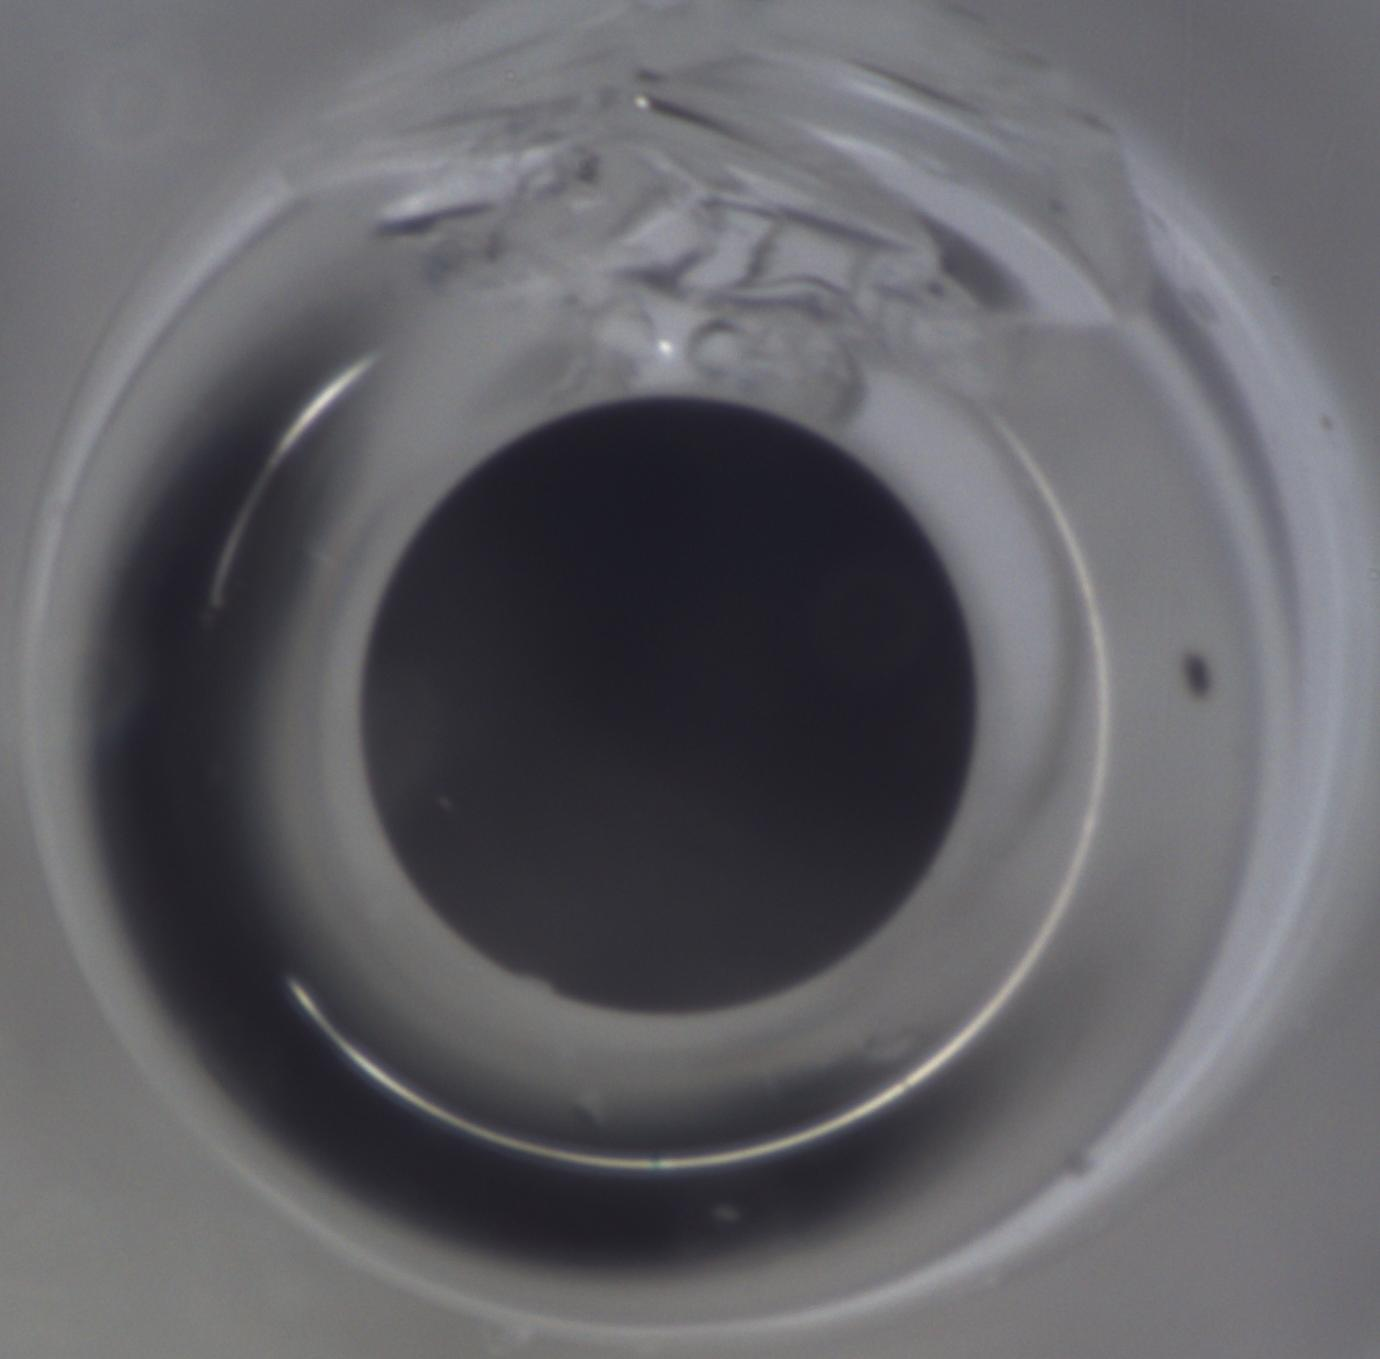
\includegraphics[width=.4\textwidth]{abbildungen/ohnelipidschicht_cut.jpg}
  \caption{"`Loch"' ohne Lipidschicht. Es befindet sich am Ende eines Rörchens, dass den inneren und äußeren Teil der Küvette verbindet.
Es erscheint schwarz, da daran kein Licht reflektiert wird.\\
Die Kreisrunde Reflexion am Rand indiziert, dass die Lichtquelle richtig eingestellt ist, um Newtonsche Ringe beim Anbringen einer
Lipidschicht zu sehen. Die folgenden Bilder der Lipidschicht sind so ausgeschnitten, dass der äußere Rand nicht mehr sichtbar ist und man nur den inneren Rand des Lochs sieht.}
  \label{fig:loch}
\end{figure}

Mit einem Teflonstäbchen wurde dann in der Elektrolytlösung eine Lipidschicht auf der Öffnung angebracht. Durch Abstreifen mit dem 
Teflonstäbchen und Durchrühren der Lösung wurde sie ausgedünnt, bis zuerst newtonsche Ringe sichtbar wurden und sich anschließend 
darin eine Lipid-Doppelschicht herausbildete, die BLM. Ein Bild von einer sich ausbreitenden BLM is in Abbildung \ref{fig:newton} zu sehen.

\begin{figure}[tbh!]
  \centering
  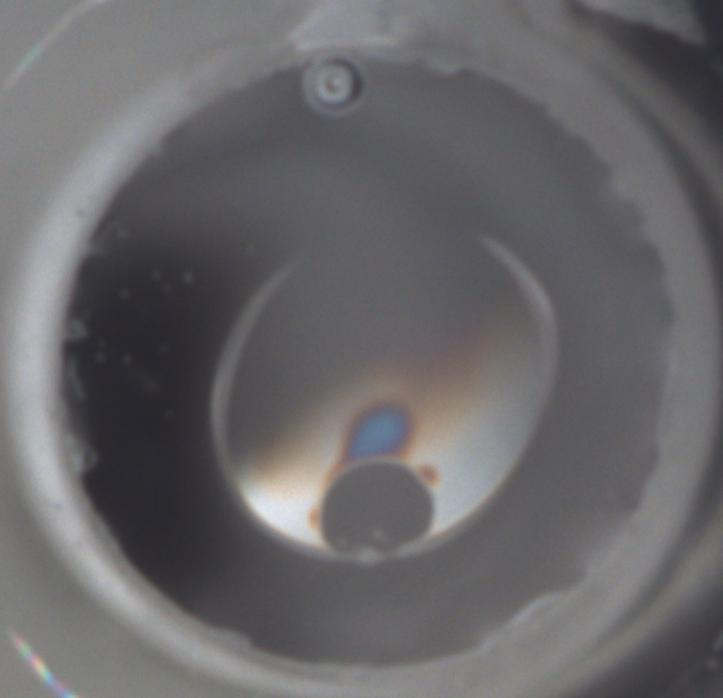
\includegraphics[width=.4\textwidth]{abbildungen/newton2_cut.jpg}
  \caption{"`Loch"' mit angebrachter Lipidschicht. Sie ist schon dünn genug, dass man Newtonsche Ringe sieht, da die Dicke im Bereich der Wellenlänge ist. Am unteren Rand ist als schwarzer Fleck die BLM zu sehen, die sich gerade herausbildet und in der Lididschicht ausbreitet.
Sie ist nun noch dünner, sodass es zu keiner Interferenz zu Newtonschen Ringen mehr kommt, weshalb sie schwarz erscheint.}
  \label{fig:newton}
\end{figure}

Für die erste Aufgabe war es wichtig, die Fläche der BLM zu kennen. Dazu haben wir ein Screenshot von der ausgebildeten BLM gemacht, wie sie 
in der Aufgabe verwendet wurde. Die Flächenbestimmung ist in Abbildung \ref{fig:blmflaeche} dargestellt und beschrieben. 
Wir erhielten daraus eine Membranfläche von 
\begin{equation} A = \SI{0,35}{mm^2}.\label{eq:area}\end{equation}
Beide Teile der Küvette enthielten jeweils eine Elektrode. An die Elektroden
wurde nun eine Rechteckspannung mit einer Frequenz von 100\,Hz angelegt. Bei jedem Umpolen der Rechteckspannung entlud sich die Membran wie ein Plattenkondensator exponentiell, bis die Spannung gegen Null ging. Die Frequenz war klein genug, dass sich die Membran fast vollständig entladen konnte, bevor es wieder zu einem Umpolen kam.\\

Auf dem Oszilloskop war sichtbar, dass die Spannungsamplitude 10\,V betrug. Wir haben nun am Oszilloskop abgelesen, nach welcher Zeitspanne die Spannung auf
\begin{equation}
 \frac{U_0}{\mathrm{e}} = \frac{\SI{10}{V}}{\mathrm{e}} \approx \SI{3,7}{V} 
\end{equation}
abfiel. Das ist die Relaxationszeit und die Betrug bei uns ungefähr

\begin{equation}
  \tau \approx \SI{60}{\micro\s}.
\end{equation}

Damit kann nun  mit dem Widerstand $R_C = \SI{100}{k\ohm}$ % bin mir hier echt nicht sicher, welcher Wid. verwendet werden muss, muss Michel fragen
über Gleichung (14) aus der Vorbereitung die Kapazität der BLM bestimmen:
e\begin{equation}
 C = \frac{\tau}{R_C} = \frac{\SI{60}{\micro\s}}{\SI{100}{k\ohm}} = \SI{0,6}{\nano\farad}.
\end{equation}

Mit der Membranfläche aus \eqref{eq:area} erhält man die spezifische Kapazität der Membran:

\begin{equation}
  C_{spez} \frac{C}{A} = \frac{\SI{0,6}{\nano\farad}}{\SI{0,0035}{cm^2}} \approx \SI{0,17}{\micro\farad\per\cm^2}.
\end{equation}

Außerdem erhält man mit einer angenommenen relativen Permittivät der Membran von $\epsilon_r = 2 $ \ref{ref:mappe},
unter Verwendung von Gleichung (12) aus der Vorbereitung 
die Membrandicke
\begin{equation}
  d = \epsilon_0 \epsilon_r \frac{A}{C} = \SI{8,85e-12}{\farad\per\m} \cdot 2 \cdot \frac{\SI{0,35e-6}{m^2}}{\SI{0,6}{nF}} 
\approx \SI{10,33}{nm}.
\end{equation}

\begin{figure}[tbh!]
  \centering
  \begin{minipage}[b]{.4\textwidth}
    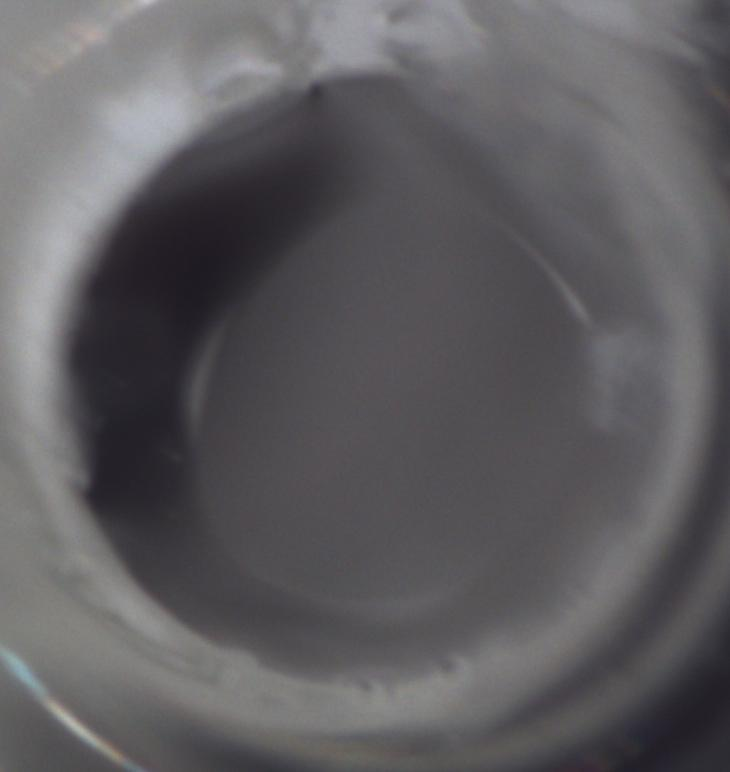
\includegraphics[width=1.\textwidth]{abbildungen/lipid5final_cut.jpg}
  \end{minipage}
  \begin{minipage}[b]{.4\textwidth}
    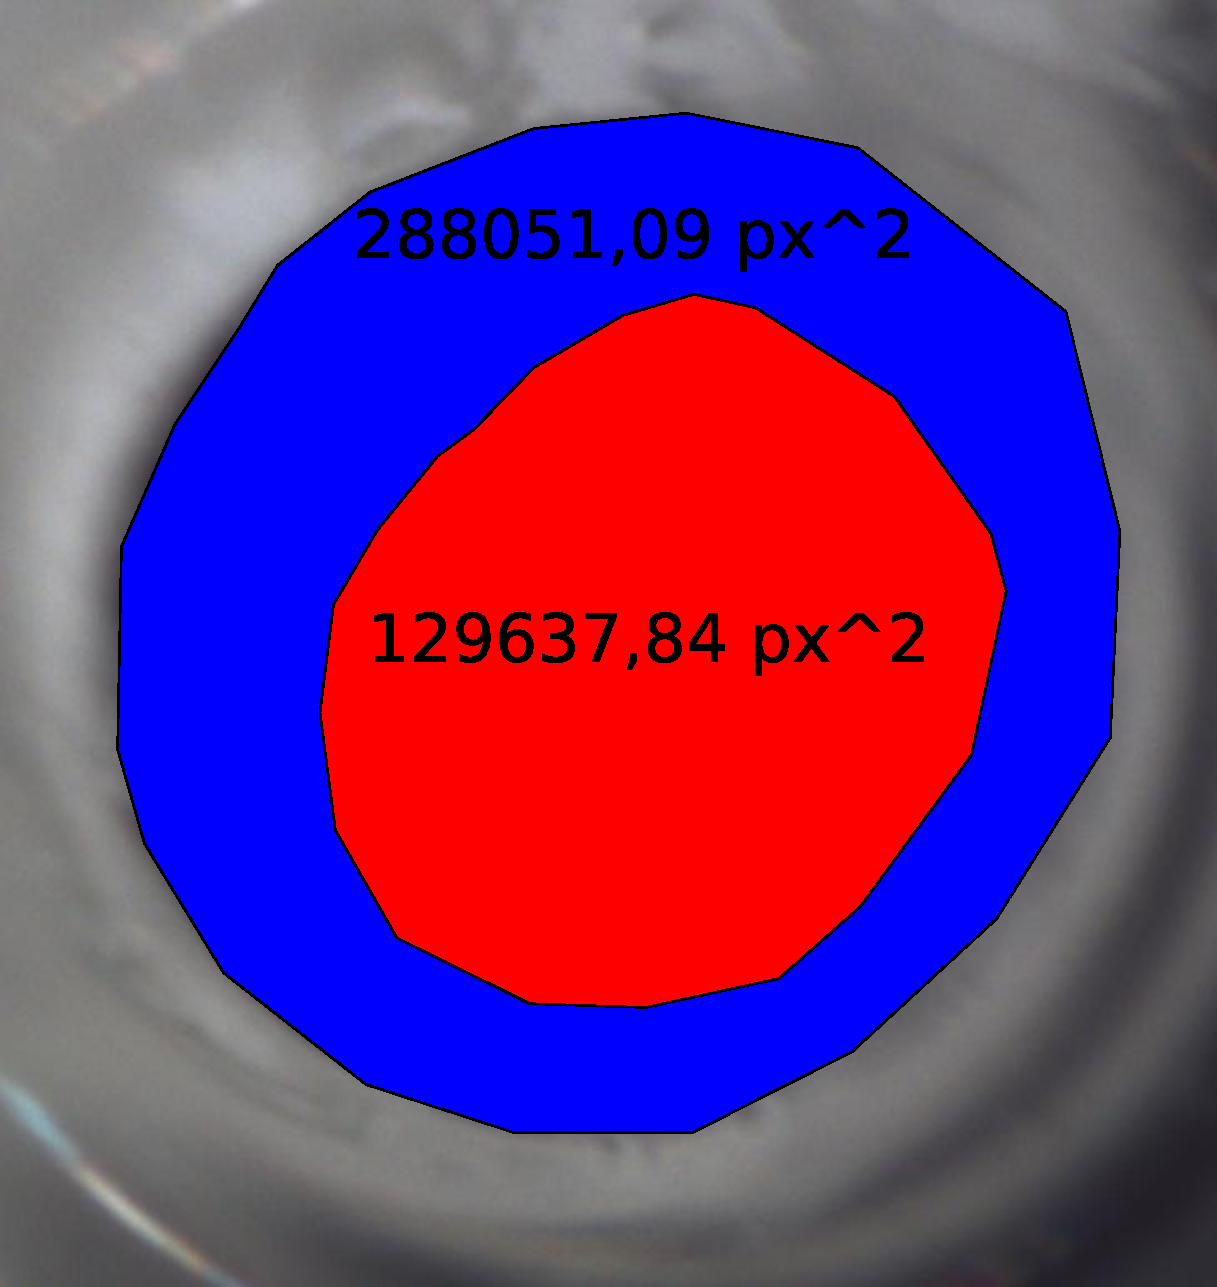
\includegraphics[width=1.\textwidth]{abbildungen/flaechenbestimmung.pdf}
  \end{minipage}
  \caption{Links ist eine vollständig ausgebildete BLM innerhalb des Lochs zu sehen.
Es ist bekannt, dass das Loch einen Durchmesser von 1\,mm. Durch Verhältnisbildung kann damit die Fläche 
der BLM bestimmt werden. Die Flächen auf dem Bilden hätten durch Bestimmung der Durchmesser abgeschätzt werden können. Da die BLM jedoch
nicht kreisförmig ist, haben wir die beiden relativen Fläche bestimmt, indem wir in dem Vektorgrafik-Programm "`Inkscape"'
jeweils um den Rand des Lochs und um die BLM Polygonpfade gelegt haben und die darin eingeschlossenen Flächen berechnen lassen haben. Die so 
berechneten relativen Flächen sind rechts zu sehen.\\
Daraus folgt, dass die BLM etwa 45\% des Lochs bedeckt, was bei einem Lochdurchmesser von 1\,mm einer Fläche von 0.35\,mm~$^2$ entspricht.}
\label{fig:blmflaeche}
\end{figure}

\section{Aufgabe 2: Messung einzelner Ionenkanäle}

\section{Aufgabe 3: Messung multipler Ionenkanäle}

\section{Aufgabe 4: Weitere Fragen}

\section{Quellen}
\begin{enumerate}
\item Vorbereitungsmappe \label{ref:mappe}
\end{enumerate}



\end{document}
